\chapter{Sumas}\label{chapter_sumas}
Realicemos la siguiente suma lo más rápido posible
\[
	1+2+3+\cdots + 97+98+99+100
\]
La forma que ideó Gauss, un gran matemático fue tomar las 50 parejas de los extremos hacia el centro que suman 101 y descubrió asi que entonces la anterior suma era
\[
50\times 101=5050
\]

\textbf{Ver video:} \url{https://www.youtube.com/watch?v=LpNHKkFSQII}
\begin{ejemplo} Hagamos ahora por ejemplo la suma
	\[
			1+2+3+\cdots + 97+98+99+100+101
	\]
	\begin{itemize}
		\item \textbf{Forma 1:} Va a sumar lo mismo anterior mas 101, es decir, $5050+101=5151$.
		
		\item \textbf{Forma 2:} Volver a hacer parejas desde los extremos que sumarán $102$ y ver que hay $50$ parejas y el número $51$ se queda sin pareja. Entonces suma
		\[
		(50\times 102 ) + 51 =5151
		\]
		
		\item \textbf{Forma 3:} (Mi favorita). Al ser impar sabemos que va  quedar faltando un número por pareja. Entonces en vez de tomar parejas desde los extremos tomemos parejas desde el 100 que es par de forma que sumen $101$ , entonces la suma será
		\[
		(\underbrace{50}_{\text{50 parejas}}\times 101 ) + 101
		\]
		
		\item \textbf{Mejor forma y la mas facil para no preocuparnos por si hay cantidad par o impar:}.
			\begin{align*}
				S&= &1&+&2&+&3&+&\cdots &+ &99&+&100&+&101\\
				S&= &101&+&100&+&99&+&\cdots&+& 3&+&2&+&1\\
				\hline\\
				2S&= &102 &+ &102 &+ &102 &+ &\cdots&+ &102 &+ &102 &+ &102
			\end{align*}
			Entonces vemos que sumar dos veces la suma de los numeros desde 1 hasta 101 es $2S=101\times 102$ entonces la suma de 1 hasta 101 es $\frac{101\times 102}{2}$.		
	\end{itemize}
\end{ejemplo}

\begin{exer}
	Realizar cada una de la siguientes sumas:
	\begin{enumerate}[label=\Alph*)]
		\item $1+2+3+\cdots +9+10$
		\item $1+ 2+ 3+ \cdots 52+ 53+ 54$.
		\item $1+ 2+ 3+ \cdots 88+ 89+ 90$.
		\item $1+ 2+ 3+ \cdots 498+ 499+ 500$.
		\item $1+ 2+ 3+ \cdots 998+ 999+ 1000$.
		\item $1+ 2+ 3+ \cdots 2018+ 2019+ 2020$.
	\end{enumerate}
\end{exer}

\begin{exer}{\ \\}
	Juan quiere inventar una máquina, donde el le diga un número y ella le calcule la suma de los números desde 1 hasta ese número. Por ejemplo, si Juan le dice a la máquina 5, la maquina le responderá: 15, pues $1+2+3+4+5=15$. La máquina de Juan se ha dañado y solo es capaz de hacer multiplicaciones y divisiones para calcular la respuesta, sin embargo Juan cree que puede arreglarla para que ella pueda seguir respondiendo acertadamente, cómo lo hace? Explica que proceso hace la máquina para lograr responderle a Juan con cualquier número que el le dice? (No te preocupes si no sabes como Juan ha arreglado la máquina, utiliza la técnica de hacer has mas ejemplos y descúbrelo!)
\end{exer}

\begin{tcolorbox}[colback=black!5!white,colframe=black]
	\textbf{Aplicando a programación:}
	\begin{itemize}
		\item Cada uno va a hacer en scratch un personaje que diga el problema y la solución. Por ejemplo, que diga: "La suma de los numeros de 1 a 100 es 5050".
		\item Ahora hacer que primero tu muñeco pida un numero, luego tu lo escribes y luego el muñeco lo diga. 
		\item Ahora hacer que primero tu muñeco pida tu edad, luego tu escribes tu edad en numero y luego el muñeco diga el doble de tu edad. 
		\item Que tu muñeco diga: "Soy muy listo! Soy capaz de calcular la suma de todos los numeros desde 1 hasta el numero que tu me digas, hasta cual quieres que sume?", luego tu ingresas un numero y finalmente tu muñeco debe dar la respuesta. Por ejemplo, si escribo 10, el muñeco debe decir "La suma da 55".
		\item Cuando lo tengas, prueba que te quedon bien aplicandolo a los ejercicios vistos anteriormente.
	\end{itemize}
\end{tcolorbox}




		
		
\begin{ejemplo}
	Queremos ahora calcular la suma 
	\[
		20+21+22+\cdots+97 + 98 +99+100
	\]
	\begin{itemize}
	\item \textbf{Forma 1:} 
	\begin{align*}
	S&= &20&+&21&+&22&+&\cdots &+ &98&+&99&+&100\\
	S&= &100&+&99&+&98&+&\cdots&+& 22&+&21&+&20\\
	\hline\\
	2S&= &120 &+ &120 &+ &120 &+ &\cdots&+ &120 &+ &120 &+ &120
	\end{align*}
	Entonces la suma es $\frac{120\times 81}{2} = 4.860$.
	
	\item \textbf{Forma 2:} Si nos damos cuenta esto es lo mismo que calcular la suma desde 1 hasta 100 y restarle la suma desde 1 hasta 19.
	\begin{align*}
	\text{Suma de 1 a 100} &= 1+2+3+\cdots +18+19 \color{black}+20+21+22+\cdots+97 + 98 +99+100 &&= 5050 \\
	-\text{  Suma de 1 a 19} &= 1+2+3+\cdots +18+19 &&= 190\\
	\hline\\
	\text{Suma de 20 a 100} &=	20+21+22+\cdots+97 + 98 +99+100 &&= 4.860		
	\end{align*}
	\end{itemize}
\end{ejemplo}


\begin{exer}
	Calcular de dos formas diferentes cada una de las siguientes sumas:
	\begin{enumerate}[label=\Alph*)]
		\item  \[33+36+39+\cdots+196+ 198+201\]
		\item  \[1000+1001+1002+\cdots+2018+ 2019+2020\]
		\item \[100+105+110+\cdots +2015+200\]
	\end{enumerate}
\end{exer}


\begin{exer}
	Cada uno crear un ejercicio de suma. Resolverlo y luego resolver el de los demas compañeros.
\end{exer}

\begin{ejemplo}{\ \\}
	\begin{enumerate}[label=\Alph*)]
		\item Carlos quiere ser coleccionista de hojas, así que su papá le regaló 20 hojas el mes pasado. Para seguir aumentando su numero de hojas en la colección, Carlos decide cada mes coleccionar dos hojas más que el mes anterior. Es decir, el proximo mes debe coleccionar 22 y asi sucesivamente. Si Carlos cumple con esto, cuántas hojas tendrá en total el mes en el que le toque coleccionar 40 hojas? 
		\item Cuántos meses tendrán que pasar para que Carlos tenga en total 2460 hojas?
	\end{enumerate}
\end{ejemplo}

\begin{exer}
	Cada uno crear un problema de suma como el anterior. Resolverlo y luego resolver el de los demas compañeros.
\end{exer}

\begin{exer}\textbf{Reto!}{\ \\}
	Juan quiere ahora una máquina, donde el le diga un dos numeros y ella le calcule la suma de los números desde el menor de esos numeros hasta el mayor de esos números. Por ejemplo, si Juan le dice a la máquina 5 y 10, la maquina le responderá: 35, pues $5+6+7+8+9=35$. Explica que proceso hace la máquina para lograr responderle a Juan con cualquier par de números que el le dice? 
\end{exer}

\begin{tcolorbox}[colback=white!5!white,colframe=green!50!black]
	\textbf{RETO:} Hacer un programa en Scratch donde el muñeco pregunte "Desde que numero quieres sumar?",  yo ingreso un numero, por ejemplo 20, luego el muñeco me vuelva a preguntar "Y hasta que numero quieres sumar?", y yo le ingreso hasta donde quiero sumar, por ejemplo hasta el 100. Finalmente el muñeco, en este ejemplo debería luego decir "Su suma es 4860". (Ver \url{https://scratch.mit.edu/projects/488842223/})
\end{tcolorbox}
\newpage
\begin{center}
	\vspace{-1cm}
	\section{Ejercicios: Sumas}\label{ejercicios_chapter_sumas}
\end{center}
\begin{enumerate}
	\item Calcular las siguientes sumas incluyedo los límites que se dan:
			\begin{multicols}{2}
			\begin{enumerate}[label=\Alph*)]
				\item 3 hasta 12
				\item 1 hasta 200					
				\item 100 hasta 900
				\item 1000 hasta 2020
			\end{enumerate}
			\end{multicols}
			
	\item (2 p.50 de \cite{creative_problem_solvind_NEGRO}). Para año nuevo Carlos se promete ahorrar en su alcancia 1 moneda el día 1 del año, 2 monedas el día 2 del año, 3 el día 3, 4 el día 4 y así sucesivamente hasta que se terminen los 365 días del año.
			\begin{enumerate}[label=\Alph*)]
			\item Cuántas monedas habrá en su alcancia cuando termine el año? 
			\item Si ahorra con monedas de 200 pesos, cuanto ahorró?
			\end{enumerate}
	
	\item (3 p.50 de \cite{creative_problem_solvind_NEGRO}).  En bolos, diez pinos se colocan al final de la pista formando un triangulo de 4 filas como muestra la figura \ref{bolospinos}. Imagine que ahora tenemos una super pista de bolos donde ponemos los pinos también en forma triangular pero ahora se forman 44 filas. Cuál sería el total de pinos que habrían en la super pista? 
	
		\begin{figure}[H]
			\centering
			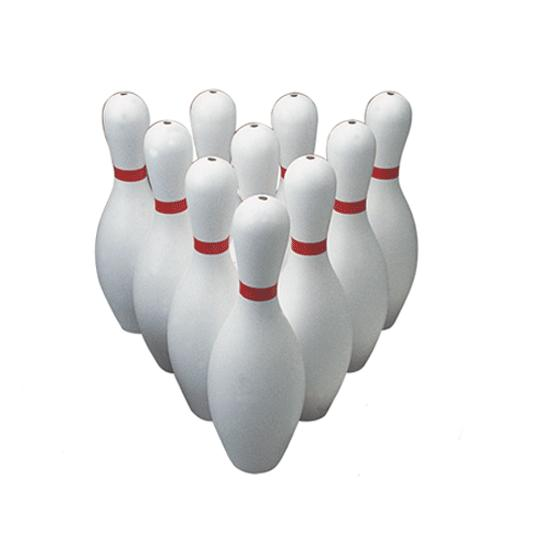
\includegraphics[width=0.4\linewidth]{TN/imgs/bolos_pinos}
			\caption{10 pinos de bolos}
			\label{bolospinos}
		\end{figure}
	
	\item (7 p.50 de \cite{creative_problem_solvind_NEGRO}). Mario organizó una fiesta en su casa. Durante la noche, el timbre de la casa sonó 20 veces. La primera vez que sonó llegó solamente un invitado. Cada vez que sonaba el timbre llegaban dos invitados mas que los invitados que habían llegado con el timbre anterior. Cuántos invitados llegaron en total a la fiesta?
	
	\item (9 p.50 de \cite{creative_problem_solvind_NEGRO}). Suponga que usted tiene un secreto. El lunes se lo cuenta a dos amigos. El martes, cada uno de estos amigos se lo cuenta a otros dos amigos. Si este procedimiento continúa día a día, cuántas personas en total sabrán su secreto hasta el siguiente domingo? 
	
	\item \textbf{Wow}. El sapo saltarín tiene afán de llegar a su casa. En el primer salto avanza $1m$, y de ahí en adelante siempre salta el doble de la distancia que saltó en el anterior salto, es decir, en el segundo salto saltará $2m$, en el tercero $4m$, en el cuarto $8m$ y así sucesivamente. Si en total realizó 20 saltos para llegar a su casa, que tan lejos estaba de su casa justo antes de dar el primer salto?
	
	\item \textbf{Wow}. Una tortuga perezosa no tiene afán de llegar a su casa. En el primer salto avanza $1m$, y de ahí en adelante siempre salta la mitad de la distancia que saltó en el anterior salto, es decir, en el segundo salto saltará $\frac{1}{2}m$, en el tercero $\frac{1}{4} m$, en el cuarto $\frac{1}{8} m$ y así sucesivamente. Si en total realizó 20 saltos para llegar a su casa, que tan lejos estaba de su casa justo antes de dar el primer salto?
	
	\item \textbf{Woww} En la Figura \ref{secuenciaCuarto} el cuadrado mas grande tiene área $1 {cm}^2$, calcular el área amarilla. (Nota: Cada cuadrado superior derecho se vidide en 4 sucesivamente sin parar)
	
		\begin{figure}[H]
			\centering
			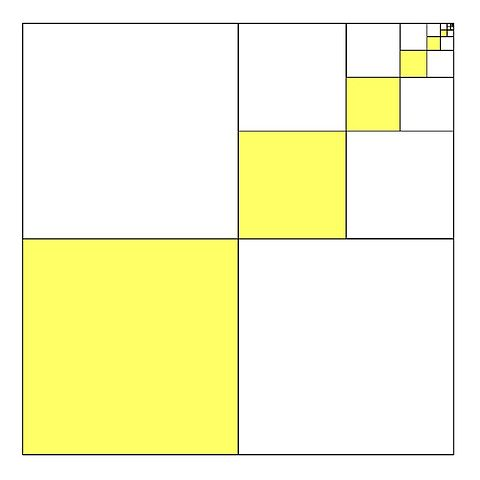
\includegraphics[width=0.4\linewidth]{TN/imgs/secuenciaCuartoEnCuarto}
			\caption{10 pinos de bolos}
			\label{secuenciaCuarto}
		\end{figure}
	
\end{enumerate}
\newpage


\begin{tcolorbox}[colback=white!5!white,colframe=green!50!black]
	Se recomienda continuar con la sección \ref{section_fact_para_calc_sumas} para ver mas sumas usando factorización.
\end{tcolorbox}

\chapter{Números Primos}
(VER DIAPOSITIVAS DIVISORES Y DIVISIBILIDAD)
Ver  \href{run:TN/Anexos/Primaria_2018_CAP1_medio_Multiplos_y_divisores_y_MCD_y_MCM.pdf}{Guía Múltiplos y divisores, Primera capacitación Nivel medio Primaria 2018}

\begin{exer}
	Escribir en una lista los números primos del 1 al 30.
\end{exer}

\begin{tcolorbox}[colback=black!5!white,colframe=black]
	Para practicar que tantos números primos conoces, accede a este link para ver cuántos primos aciertas en 1 minuto:
	
	\centering
	\url{https://isthisprime.com/game/}
\end{tcolorbox}

\section{Descomposición en Primos}
\begin{ejemplo} La idea es dividir al 60 por el número primo mas pequeño que se pueda, este es 2, así $60=2\times 30$. Luego hacer lo mismo con el número que no es primo, o sea 30. El primo mas pequeño que lo divide es 2, así $60=2\times 30=2\times 2\times 15$. Como 15 no es primo seguimos, $60=2\times 30=2\times 2\times 15=2\times 2\times3\times 5$. Acá nos detenemos pues ya todos los números que tenemos son primos. Este proceso que se hizo se puede ver mejor en un diagrama (Ver \ref{descomposicionenfactores60}).
	
	\begin{figure}[htbp]
		\centering
		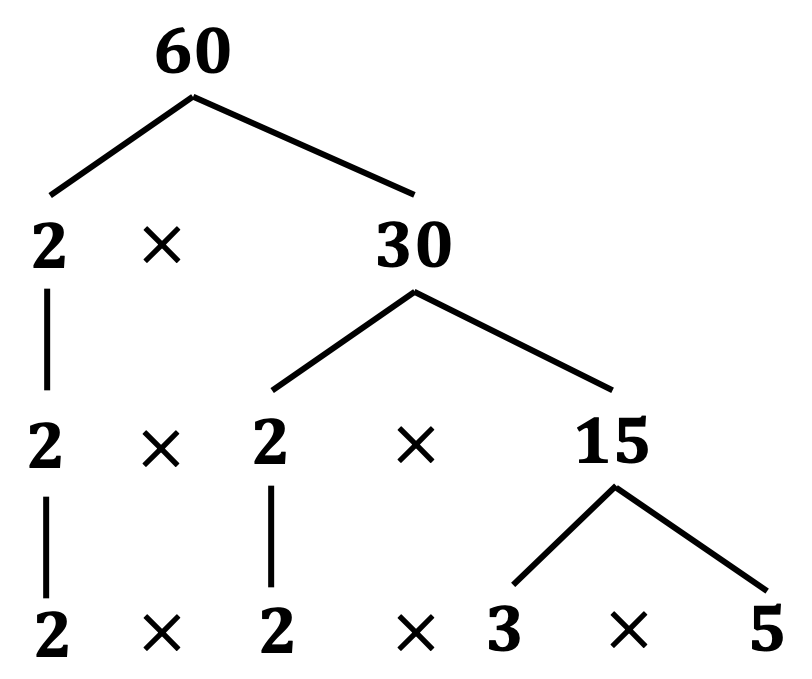
\includegraphics[width=90mm]{TN/imgs/descomposicion_en_factores_60}
		%\caption{}
		\label{descomposicionenfactores60}
	\end{figure}
	
	\begin{exer}
		Descomponer al número 48 en factores primos.
	\end{exer}
	
	\begin{exer}
		Hacer la descoomposición en factores primos de los siguientes números:
		\begin{multicols}{3}
			\begin{enumerate}[label={\alph*})]
				\item 6
				\item 78
				\item 15
				\item 24
				\item 49
				\item 360
				\item 510
				\item 900
				\item 144
				\item 250
				\item 36
			\end{enumerate}
		\end{multicols}
	\end{exer}
\end{ejemplo}

\textbf{\textcolor{red}{Pregunta.}}  Si tuvieramos que la descomposición de dos números son las siguientes
\[
2\times 2\times 3\times 3\times 5\times 5
\]
y
\[
2\times  3\times 3\times 5\times 7
\]
Cómo haría para encontrar el \textbf{mínimo común múltiplo} y el \textbf{máximo común divisor}?

\newpage
Actividad Decomposición en factores primos. Tomado de “Math in Focus curso 1 A”.
\textsl{}